    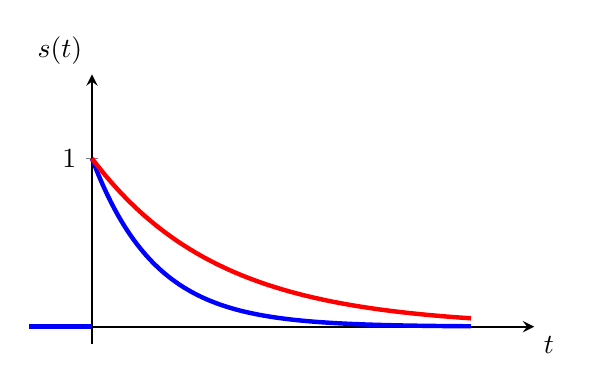
\begin{tikzpicture}
        \begin{axis}[
        axis line style = thick,
%        clip=false,
        height=5cm,
        width=8cm,
        axis x line=center,
        axis y line=center,
        xmin=-1,
        xmax=7,
        ymin=-0.1,
        ymax=1.5,
        xlabel={$t$},
        ylabel={$s(t)$},
        xlabel style={below right},
        ylabel style={above left},
        ytick={1},
        yticklabels={$1$},
        xtick=\empty,
        ]
            \addplot [ultra thick,color=blue,domain=-1:0, samples=101,unbounded coords=jump]{0};
            \addplot [ultra thick,color=blue,domain=0:6, samples=101,unbounded coords=jump]{exp(-x)};
            \addplot [ultra thick,color=red,domain=0:6, samples=101,unbounded coords=jump] {exp(-0.5*x)};
        \end{axis}
    \end{tikzpicture}
